\documentclass[preview]{standalone}
\usepackage{tikz,fullpage,tikz-network,verbatim}
\usetikzlibrary{arrows, petri, topaths, calc, angles, quotes}
\begin{document}
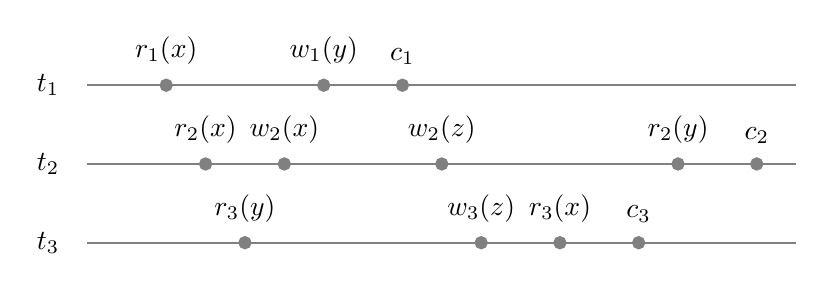
\begin{tikzpicture}[scale=1,transform shape,
>={Stealth[round]},thick,black!50,text=black,
every new ->/.style={shorten >=1pt},
graphs/every graph/.style={edges=rounded corners}]

  % \draw (0, 0) grid (10, 5);
  
  % \draw (0.5, 4) node {$t_0$} (1, 4) -- (10, 4) node { };
  \draw (0.5, 3) node {$t_1$} (1, 3) -- (10, 3) node { };
  \draw (0.5, 2) node {$t_2$} (1, 2) -- (10, 2) node { };
  \draw (0.5, 1) node {$t_3$} (1, 1) -- (10, 1) node { };
 
  % s = r_1(x) r_2(x) r_3(y) w_2(x) w_1(y) c_1 w_2(z) w_3(z) r_3(x) c_3 r_2(y) c_2 
  \coordinate (w0x) at (0  ,4);
  \coordinate (w0y) at (0  ,4);
  \coordinate (c0)  at (1  ,4);
  \coordinate (r1x) at (2  ,3);
  \coordinate (r2x) at (2.5,2);
  \coordinate (r3y) at (3  ,1);
  \coordinate (w2x) at (3.5,2);
  \coordinate (w1y) at (4  ,3);
  \coordinate (c1)  at (5  ,3);
  \coordinate (w2z) at (5.5,2);
  \coordinate (w3z) at (6  ,1);
  \coordinate (r3x) at (7  ,1);
  \coordinate (c3)  at (8  ,1);
  \coordinate (r2y) at (8.5,2);
  \coordinate (c2)  at (9.5,2);

  % step graph
  \filldraw (r1x) circle [radius=2pt] node [label=above:$r_1(x)$] {};
  \filldraw (r2x) circle [radius=2pt] node [label=above:$r_2(x)$] {};
  \filldraw (r3y) circle [radius=2pt] node [label=above:$r_3(y)$] {};
  \filldraw (w2x) circle [radius=2pt] node [label=above:$w_2(x)$] {};
  \filldraw (w1y) circle [radius=2pt] node [label=above:$w_1(y)$] {};
  \filldraw (c1)  circle [radius=2pt] node [label=above:$c_1$] {};
  \filldraw (w2z) circle [radius=2pt] node [label=above:$w_2(z)$] {};
  \filldraw (w3z) circle [radius=2pt] node [label=above:$w_3(z)$] {};
  \filldraw (r3x) circle [radius=2pt] node [label=above:$r_3(x)$] {};
  \filldraw (c3)  circle [radius=2pt] node [label=above:$c_3$] {};
  \filldraw (r2y) circle [radius=2pt] node [label=above:$r_2(y)$] {};
  \filldraw (c2)  circle [radius=2pt] node [label=above:$c_2$] {};
\end{tikzpicture}
\end{document}
